\documentclass[10pt]{amsproc}
\usepackage{graphicx,hyperref,color,ytableau}
\newtheorem{theorem}{Theorem}[subsection]
\newtheorem{lemma}[theorem]{Lemma}
\newtheorem{corollary}[theorem]{Corollary}
\theoremstyle{definition}
\newtheorem{definition}[theorem]{Definition}
\theoremstyle{remark}
\newtheorem{remark}[theorem]{Remark}
\newtheorem{example}[theorem]{Example}
\newtheorem{exercise}[theorem]{Exercise}
\newcommand{\rowins}{\mathrm{RINS}}
\newcommand{\ins}{\mathrm{INSERT}}
\newcommand{\del}{\mathrm{DELETE}}
\newcommand{\Tab}{\mathrm{Tab}}
\newcommand{\rc}[1]{\mathbf{#1}}
\newcommand{\rd}{\mathrm{read}}
\newcommand{\wt}{\mathrm{wt}}
\newcommand{\shape}{\mathrm{shape}}
\newcommand{\pl}{\mathrm{pl}}
\newcommand{\ttab}{\mathrm{tt}}
\newcommand{\tr}{\mathrm{tR}}
\newcommand{\rp}{\mathbf{R}^+}
\newcommand{\rsk}{\mathrm{RSK}}
\newcommand{\ot}{\leftarrow}
\newcommand{\infl}{\mathrm{INFL}}
\title{Knuth's moves on Timed Words}
\author{Amritanshu Prasad}
\address{The Institute of Mathematical Sciences, Chennai}
\address{Homi Bhabha National Institute, Mumbai}
\begin{document}
\maketitle
\ytableausetup{smalltableaux}
\section{Schensted's Algorithm}
\label{sec:intro}
\subsection{Words}
\label{sec:words}
Let $A_n$ denote the set $\{1,\dotsc,n\}$, which we regard as an \emph{ordered alphabet}.
A \emph{word} in $A_n$ is a finite sequence $w=c_1\dotsb c_k$ of elements of $A_n$.
The set of all words in $A_n$ is denoted $A_n^*$.
A \emph{subword} of $w=c_1\dotsb c_k$ is defined to be a word of the form
\begin{displaymath}
  w' = c_{i_1}\dotsb c_{i_m}, \text{ where } 1\leq i_1 < \dotsb < i_m \leq k.
\end{displaymath}
The subword $w'$ is said to be \emph{weakly increasing} if $c_{i_1}\leq \dotsb \leq c_{i_m}$.

Consider the following computational problem:
\begin{quote}
  Given a word $w\in A_n^*$, determine the maximal length of an increasing subword of $w$.
\end{quote}
\subsection{Tableaux}
Schensted~\cite{schensted} gave an elegant algorithm to solve the preceding computational problem.
His algorithm makes one pass over the word.
At each stage of its running, it stores a combinatorial object called a \emph{semistandard Young tableau} (see Section~\ref{definition:ssyt}) which is modified as each successive letter of the word is read.
The length of the longest increasing subword can be read off from the tableau (see Sections~\ref{sec:insert-tabl-word} and~\ref{sec:schensted-theorem}) obtained when all of $w$ has been read.

\begin{definition}
  [Semistandard Young Tableau]
  \label{definition:ssyt}
  A semistandard Young \linebreak tableau in $A_n$ is a finite arrangement of integers from $A_n$ in rows and columns so that the numbers increase weakly along rows, strictly along columns, so that there is an element in the first row of each column, there is an element in the first column of each row, and there are no gaps between numbers.

  Let $l$ be the number of rows in the tableau, and for each $i=1,\dotsc,l$, let $\lambda_i$ be the length of the $i$th row.
  Then $\lambda=(\lambda_1,\dotsc,\lambda_l)$ is called the \emph{shape} of the tableau.
\end{definition}
\begin{example}
  \label{example:ssyt}
  The arrangement
  \begin{displaymath}
    \ytableaushort{115,24,3}
  \end{displaymath}
  is a semistandard Young tableau of shape $(3,2,1)$ in $A_5$.
\end{example}

The notion of a semistandard Young tableau is a generalization of \emph{Young tableau}, which was introduced by Young~\cite[p.~133]{doi:10.1112/plms/s1-33.1.97} during the course of his investigations into the representation theory of the symmetric group (which he called \emph{substitutional analysis}).
In Young's version, each element of $A_n$ occurs exactly once in the tableau.
For brevity, we shall henceforth use the term \emph{tableau} to refer to a \emph{semistandard Young tableau}.
\subsection{Row Insertion}
\label{sec:row-insertion}A row of length $k$ is defined to be a weakly increasing sequence $u=a_1a_2\dotsb a_k$ in $A_n$.
Let $R(A_n)$ denote the set of all rows in $A_n$.
Each row of a tableau is a row in the sense of this definition.
For each $u=a_1\dotsb a_k\in R(A_n)$ and $a\in A_n$, define the row insertion of $a$ into $u$ by:
\begin{displaymath}
  \rowins(u,a) =
  \begin{cases}
    (\emptyset, a_1\dotsb a_k a) & \text{if } a_k\leq a,\\
    (a_j,a_1\dotsb a_{j-1}aa_{j+1}\dotsb a_k) & \text{otherwise, with}\\
    & j=\min\{i\mid a<a_i\}.
  \end{cases}
\end{displaymath}
Here $\emptyset$ should be thought of as an empty row of length zero.
\begin{example}
  $\rowins(115,5) = (\emptyset,1155)$, $\rowins(115,3)=(5,113)$.
\end{example}
It is clear from the construction that, for any $u\in R(A_n)$ and $a\in A_n$, if $(a',u')=\rowins(u,a)$, then $u'$ is again a row.
For convenience set $\rowins(u,\emptyset)=(\emptyset,u)$.
\subsection{Tableau Insertion}
\label{sec:tableau-insertion}
Let $t$ be a tableau with rows $u_1,u_2,\dotsc, u_l$.
Then $\ins(t,a)$, the insertion of $a$ into $t$, is defined as follows: first $a$ is inserted into $u_1$; if $\rowins(u_1,a)=(a_1',u_1')$, then $u_1$ is replaced by $u_1'$.
Then $a_1'$ is inserted into $u_2$; if $\rowins(u_2,a_1')=(a_2',u_3)$, then $u_2$ is replaced by $u_2'$, $a_2'$ is inserted into $u_3$, and so on.
This process continues, generating $a_1',a_2',\dotsc,a_k'$ and $u_1',\dotsc,u_k'$.
The tableau $t'=\ins(t,a)$ has rows $u_1',\dotsc,u_k'$, and a last row (possibly empty) consisting of $a_k'$.
It turns out that $\ins(t,a)$ is a tableau \cite{knuth}.
\begin{example}
  \label{example:insertion}
  For $t$ as in Example~\ref{example:ssyt}, we have
  \begin{displaymath}
    \ins(t,3) = \ytableaushort{113,245,3},
  \end{displaymath}
  since $\rowins(115,3)=(5,113)$, $\rowins(24,5)=(\emptyset,245)$.
\end{example}
\subsection{Insertion Tableau of a Word}
\label{sec:insert-tabl-word}
An arbitrary sequence $a_1\dotsb a_k$ in $A_n$ will be called a word in $A_n$.
The set of all words in $A_n$ is denoted by $A_n^*$.
This set may be regarded as a monoid under concatenation, with identity element as the empty word, denoted by $\emptyset$.
\begin{definition}
\label{definition:insertion-tableau}
The insertion tableau $P(w)$ of a word $w$ is defined recursively as:
\begin{align}
  P(\emptyset)&=\emptyset\\
  P(c_1\dotsb c_k)&=\ins(P(c_1\dotsb c_{k-1}), c_k).
\end{align}
\end{definition}
\begin{example}
  \label{example:insertion-tableau}
  Take $w=3421153$.
  Sequentially inserting the terms of $w$ into the empty tableau $\emptyset$ gives the sequence of tableaux:
  \begin{displaymath}
    \ytableaushort{3},\ytableaushort{34},\ytableaushort{24,3},\ytableaushort{14,2,3},\ytableaushort{11,24,3},\ytableaushort{115,24,3},
  \end{displaymath}
  and finally, the insertion tableau $P(w)=\ytableaushort{113,245,3}$.
\end{example}
\subsection{Schensted's Theorem}
\label{sec:schensted-theorem}
Schensted's proved the following theorem:
\begin{theorem}
  The length of the longest increasing subword of any $w\in A_n^*$ is the length of the first row of $P(w)$.
\end{theorem}
In other words, the algorithm for constructing the insertion tableau of $w$ solves the computational problem posed in Section~\ref{sec:words}.

The proof of Schensted's theorem is not very difficult, and the reader is invited to attempt it.
The proof is by induction on $k$, and uses the observation is that the last entry of the first row of $P(a_1\dotsb a_k)$ is the \emph{least last element} of all maximal length weakly increasing subword of $a_1\dotsb a_k$.
\subsection{Greene's Theorem}
\label{sec:greenes-theorem}
The insertion tableau $P(w)$ obtained from a word $w$ seems to contain a lot more information tham just the length of the longest weakly increasing subword.
For example, what do the lengths of the remaining rows of $P(w)$ signify?
The answer to this question was given by Greene~\cite{Greene-schen}.
We say that subwords $c_{1_1}\dotsb c_{i_r}$ and $c_{j_1}\dotsb c_{j_s}$ are \emph{disjoint} if the subsets $\{i_1,\dotsc,i_r\}$ and $\{j_1,\dotsc,j_s\}$ are disjoint.
\begin{definition}
  [Greene Invariants]
  The $r$th Greene invariant of a word $w\in A_n^*$ is defined to be the maximum cardinality of a union of $k$ pairwise disjoint weakly increasing subwords of $w$.
\end{definition}
\begin{example}
  \label{example:greene}
  For $w=3421153$, the longest weakly increasing subwords have length $3$ (for example, $113$ and $345$).
  The subwords $345$ and $113$ are disjoint, and no pair of disjoint weakly increasing subwords of $w$ can have cardinality greater than $6$.
  However, the entire word $w$ is a union of three disjoint weakly increasing subwords (for example $345$, $23$ and $15$).
  So the Greene invariants of $w$ are $a_1(w)=3$, $a_2(w)=6$, and $a_3(w)=7$.
\end{example}
\begin{theorem}
  [Greene]
  \label{theorem:greene}
  For any $w\in A_n$, if $P(w)$ has shape $\lambda=(\lambda_1,\dotsc, \lambda_l)$, then for each $r=1,\dotsc,l$, $a_r(w)=\lambda_1+\dotsb + \lambda_l$.
\end{theorem}
Example~\ref{example:greene} is consistent with Greene's theorem as the shape of $P(w)$ is $(3, 3, 1)$ and the Greene invariants are $3$, $6=3+3$ and $7=3+3+1$, respectively.

\subsection{Knuth Equivalence}
\label{sec:knuth-equivalence}

Greene's proof of Theorem~\ref{theorem:greene} is based on the notion of Knuth equivalence.
Knuth \cite{knuth} identified a pair of elementary moves on words:
\begin{gather}
  \tag{$K1$}\label{eq:k1}
  xzy \equiv zxy \text{ if } x\leq y < z,
  \\
  \tag{$K2$}\label{eq:k2}
  yxz \equiv yzx \text{ if } x < y \leq z.
\end{gather}
For example, in the word $4213443$, the segment $213$ is of the form $yxz$, with $x<y\leq z$.
A knuth move of type (\ref{eq:k2}) replaces this segment by $yzx$, which is $231$.
Thus a Knuth move of type (\ref{eq:k2}) transforms $4\textbf{213}443$ into $4\textbf{231}443$.
Knuth equivalence is the equivalence relation on $A_n^*$ generated by Knuth moves:
\begin{definition}[Knuth Equvalence]
  \label{definition:Knuth-equiv}
  Words $w,w'\in A_n^*$ are said to be Knuth equivalent if $w$ can be transformed into $w'$ by a series of Knuth moves (\ref{eq:k1}) and (\ref{eq:k2}).
  If this happens, we write $w\equiv w'$.
\end{definition}
\begin{example}
  \label{example:knuth-red}
  The word $3421153$ is Knuth equivalent to $3245113$:
  \begin{displaymath}
    \textbf{342}1153 \equiv_{K2} 3\textbf{241}153 \equiv_{K2} 32\textbf{141}53 \equiv_{K1} 3241\textbf{153} \equiv_{K1} 324\textbf{151}3 \equiv_{K1} 3245113.
  \end{displaymath}
  At each stage, the letters to which the Knuth moves will be applied to obtain the next stage are highlighted.
\end{example}
\subsection{Reading Word of a Tableau}
\label{sec:reading-word}
Givem a tableau, its reading word is obtained by reading its rows from left to right, starting with the bottom row, and moving up to its first row.
\begin{example}
  \label{example:reading-word}
  The reading word of the tableau:
  \begin{displaymath}
    \ytableaushort{113,245,3}
  \end{displaymath}
  is $3245113$.
\end{example}
\begin{exercise}
  Show that every tableau is the insertion tableau of its reading word.
\end{exercise}
\subsection{Proof of Greene's Theorem}
\label{sec:proof-greene}
The proof of Greene's theorem is based on three observations, all fairly easy to prove:
\begin{enumerate}
\item If $w$ is the reading word of a tableau of shape $\lambda=(\lambda_1,\dotsc,\lambda_l)$, then $a_r(w)=\lambda_1+\dotsb + \lambda_r$ for $r=1,\dotsc,l$.
\item Every word is Knuth equivalent to the reading word of its insertion tableau.
\item Greene invariants remain unchanged under Knuth moves.
\end{enumerate}
We illustrate these points with examples (for detailed proofs, see Lascoux, Leclerc and Thibon~\cite{Lascoux}, or Fulton \cite{fultonyt}).
For the first point, in Example~\ref{example:reading-word} the first $k$ rows of the tableau
\begin{displaymath}
  \ytableaushort{113,245,3}
\end{displaymath}
are indeed disjoint weakly increasing subwords of its reading word of maximal cardinality.
For the second point, observe that the sequence of Knuth moves in Example~\ref{example:knuth-red} transform $3421153$ to the reading word of its insertion tableau.
For the third point, consider the case of the Knuth move (\ref{eq:k1}).
A word of the from $w=uxzyv$ is transformed into the word $w'=uzxyv$.
The only issue is that a weakly increasing subword $g$ of $w$ may contain both the letters $x$ and $z$.
Then it no longer remains a weakly increasing subword of $w'$.
However, the subword, being weakly increasing, cannot contain $y$, so the $z$ can be swapped for a $y$.
This could be a problem if $y$ is part of another weakly increasing subword $g'$ in a collection of pairwise disjoint weakly increasing subwords.
In that case, we have $g=g_1xzg_2$ and $g'=g'_1y g'_2$.
We may replace them with $g_1xyg'_2$ and $g_1'zg_2$, which would still be weakly increasing, and would have the same total length as $g$ and $g'$.
\subsection{Characterization of Knuth Equivalence}
\label{sec:characterization}
Knuth equivalence can be characterized in terms of Greene invariants (see \cite[Theorem~2.15]{plaxique}).
\begin{theorem}
  Two words $w$ and $w'$ in $A_n^*$ are Knuth equivalent if and only if $a_k(uwv)=a_k(uw'v)$ for all words $u$ and $v$ in $A_n^*$.
\end{theorem}
\section{Timed Words}
\subsection{From Words to Timed Words}
\label{sec:timed-words}
\label{sec:words-to-timed-words}
Words, in the sense of Section~\ref{sec:intro}, play an important role in computer science, specifically in the formal verification of systems.
Each letter of the alphabet is thought of as an event.
A sequence of events it then nothing but a word in $A_n^*$.
The system has a starting state, and each time an event occurs, its state changes, depending both, on its current state, and the event that has occured.
Following the groundbreaking work of Rabin and Scott \cite{rabin1959finite}, finite state automata are widely used to model and formally verify the integrity of systems.

For many real-time systems, such as controllers of washing machines, industrial processes, and air or railway traffic control, the \emph{time gaps} between the occurences of the events modeled by words are as important as the events themselves.

To deal with real-time systems, Alur and Dill \cite{alur-dill} developed the theory of \emph{timed automata}.
A timed automaton responds to a sequence of events that come with time stamps for their occurence.
We introduce a finite variant of the notion of timed word that was used by Alur and Dill:
\begin{definition}
  [Timed Word]
  \label{definition:timed-word}
  A timed word in $A_n$ is a sequence of the form:
  \begin{displaymath}
    w=c_1^{t_1} c_2^{t_2}\dotsb c_k^{t_k},
  \end{displaymath}
  where $c_1,\dotsc,c_k\in A_n$, and $t_1,\dotsc,t_k$ are positive real numbers.
  The length of the timed word $w$ above is $l(w)=t_1+\dotsb+t_k$.
\end{definition}
The timed word $w$ above may also be regarded as a piecewise constant left-continuos funtion $\mathbf w:[0,l(w))\to A_n$, where
\begin{displaymath}
  \mathbf w(t) = c_i \text{ if } t_1+\dotsb+t_{i-1}\leq t < t_1+\dotsb + t_i.
\end{displaymath}
The function $\mathbf w:[0, l(w))\to A_n$ is called the \emph{function associated to the timed word $w$}.
\begin{example}
  \label{example:timed-word}
  An example of a timed word in $A_6^\dagger$ of length $7.19$ is:
  \begin{displaymath}
    w = 3^{0.82}5^{0.08}2^{0.45}6^{0.64}5^{0.94}1^{0.15}5^{0.09}1^{0.52}4^{0.29}1^{0.59}3^{0.97}4^{0.42}2^{0.61}1^{0.07}4^{0.55}
  \end{displaymath}
  Using a colormap to represent the integers $1$ to $6$,
  \begin{center}
    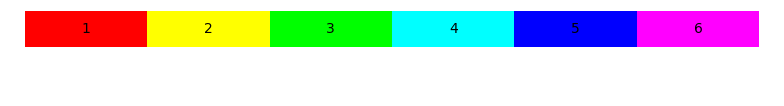
\includegraphics[width=0.85\textwidth]{colormap.png}
  \end{center}
  the timed word $w$ can be represented as a colored ribbon:
  \begin{center}
    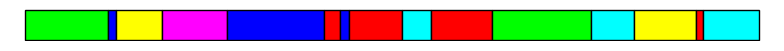
\includegraphics[width=\textwidth]{word.png}.
  \end{center}
\end{example}
\subsection{Subwords of Timed Words}
\label{sec:subwords-timed-words}
\begin{definition}
  [Time Sample]
  A \emph{time sample} of a word $w$ is a subset of $[0,l(w))$ of the form:
  \begin{displaymath}
    S = [a_1,b_1)\cup \dotsb \cup [a_k,b_k),
  \end{displaymath}
  where $0\leq a_1 < b_1 < a_2 < b_2 < \dotsb <a_k < b_k \leq l(w)$.
  The length of the time sample $S$ is defined as $l(S)=\sum_i (b_i-a_i)$, the Lebesgue measure $\mu(S)$ of $S$.
\end{definition}
Given a time sample $S\subset [0, l(w))$, and $0\leq t\leq l(S))$, there exists a unique $\tilde t\in [0, l(S))$ such that
\begin{displaymath}
  \mu(S\cap [0,\tilde t)) = t.
\end{displaymath}
Indeed, the function $t'\mapsto \mu(S\cap [0,t'))$ is a continuous function on $[0,l(w)]$ which takes value $0$ at $0$, and $l(S)$ at $1$, so by the intermediate value theorem, must take value $t$ for some $\tilde t \in [0, l(w))$. 
\begin{definition}
  [Subword of a Timed Word]
  \label{definition:timed-subword}
  The subword of a timed word with respect to a time sample $S\subset [0, l(w))$ is the timed word $w_S$ whose associated function is given by:
  \begin{displaymath}
    \mathbf w_S(t) =  \mathbf w(\tilde t),
  \end{displaymath}
  where $\tilde t\in [0,l(w))$ satisfies $\mu(S\cap [0, \tilde t)) = t$.
\end{definition}
\subsection{Timed Tableau}
\label{sec:Timed-Tableau}
\begin{definition}
  [Timed Tableau]
  \label{definition:timed-tableau}
  A timed tableau is a collection $u_1,u_2,\dotsc, u_l$ of timed words such that
  \begin{enumerate}
  \item Each associated function $\mathbf u_i$ is weakly increasing.
  \item For each $i=1,\dotsc,l-1$, $l(u_i)\geq l(u_{i+1})$.
  \item For each $i=1,\dotsc,l-1$ and $0\leq t<l(u_{i+1})$, 
  \end{enumerate}
\end{definition}
\begin{example}
  A timed tableau of shape $(3.20,1.93,1.09,0.61,0.29,0.07)$ is given by:
  \begin{align*}
    t = & 1^{1.33}2^{0.54}3^{0.36}4^{0.97}\\
    & 2^{0.52}3^{0.91}5^{0.50}\\
    &3^{0.52}4^{0.22}5^{0.32}6^{0.03}\\
    &4^{0.07}5^{0.22}6^{0.32}\\
    &5^{0.07}6^{0.22}\\
    &6^{0.07}
  \end{align*}
  In using the colormap from Section~\ref{sec:timed-words}, it can be visualized as:
  \begin{center}
    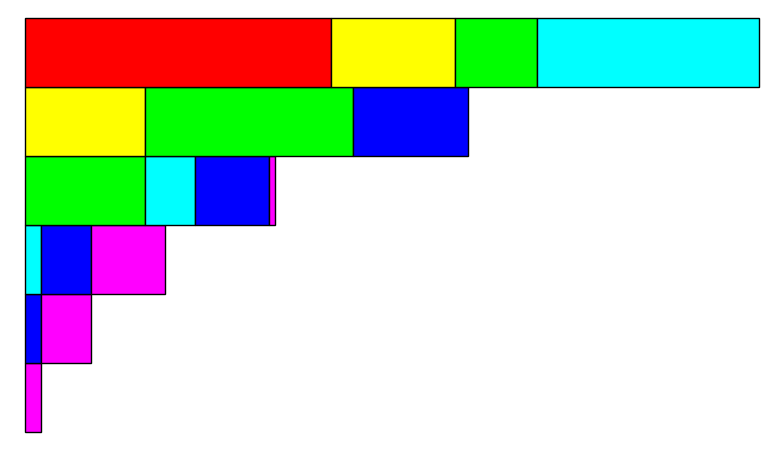
\includegraphics[width=0.5\textwidth]{tableau.png}
  \end{center}
  From the figure the three properties of Definition \ref{definition:timed-tableau} are immediately evident.
\end{example}
\subsection{Insertion for Timed Words}
\label{sec:insertion-timed-words}
\subsection{Timed Insertion}
\label{sec:timed-insertion}
Given a timed word $w$ and $0\leq a < b \leq l(w)$, according to Definition~\ref{definition:timed-subword}, $w_{[a, b)}$ is the timed word of length $b-a$ such that:
\begin{displaymath}
  w_{[a, b)}(t) = w(a+ t) \text{ for } 0\leq t<b-a.
\end{displaymath}
We call $w_{[a,b)}$ a segment of $w$.
If $a=0$, then $w_{[a,b)}$ is called an initial segment of $w$.
\begin{definition}[Timed row insertion]
  \label{definition:timed-row-insertion}
  Given a timed row $w$, define the insertion $\rowins(w, c^{t_c})$ of $c^{t_c}$ into $w$ as follows: if $w(t)\leq c$ for all $0\leq t < l(u)$, then
  \begin{displaymath}
    \rowins(w, c^{t_c}) = (\emptyset, wc^{t_c}).
  \end{displaymath}
  Otherwise, there exists $0\leq t < l(u)$ such that $w(t)>c$.
  Let
  \begin{displaymath}
    t_0 = \min\{0\leq t< u(l)\mid w(t)> c\}.
  \end{displaymath}
  Define
  \begin{displaymath}
    \rowins(w, c^{t_c}) =
    \begin{cases}
      (w_{[t_0, t_0+t_c)}, w_{[0, t_0)}c^{t_c} w_{[t_0+t_c, l(w))}) & \text{if } l(u) - t_0 > t_c,\\
      (w_{[t_0, l(u))}, w_{[0, t_0)} c^{t_c}) & \text{if } l(u) - t_0 \leq t_c.
    \end{cases}
  \end{displaymath}
  It is obvious that the above definition is compatible with the definition of $\rowins$ from Section~\ref{sec:tableau-insertion} when $u$ is a row in $A_n^*$, and $t_c=1$.
  If $u$ is a row of the form $c_1^{t_1}\dotsb c_l^{t_l}$.
  Define $\rowins(w,u)$ by induction on $l$ as follows:
  Having defined $(v',w')=\rowins(w,c_1^{t_1}\dotsb c_{l-1}^{t_{l-1}})$,
  let $(v'',w'')=\rowins(w',c_l^{t_l})$.
  Then define
  \begin{displaymath}
    \rowins(w,u) = (v'v'', w'').
  \end{displaymath}
\end{definition}
\begin{example}
  \label{example:timed-row-ins}
  $\rowins(1^{1.4}2^{1.6}3^{0.7},1^{0.7}2^{0.2})=(2^{0.7}3^{0.2},1^{2.1}2^{1.1}3^{0.5})$.
\end{example}
\begin{definition}
  [Timed Tableau Insertion]
  Let $w$ be a timed tableau with row decomposition $u_l\dotsc u_1$, and let $v$ be a timed row.
  Then $\ins(w, v)$, the insertion of $v$ into $w$ is defined as follows:
  first $v$ is inserted into $u_1$.
  If $\rowins(u_1,v)=(v_1',u_1')$, then $v_1'$ is inserted into $u_2$; if $\rowins(u_2,v_1')=(v_2',u_2')$, then $v_2'$ is inserted in $u_3$, and so on.
  This process continues, generating $v_1',\dotsc,v_l'$ and $u_1',\dotsc,u_l'$.
  $\ins(t,v)$ is defined to be $v_l'u_l'\dotsb u_1'$.
  Note that it is quite possible that $v_l'=\emptyset$.
\end{definition}
\begin{example}
  If $w$ is the timed tableau from Example~\ref{example:timed-tableau}, then
  \begin{displaymath}
    \ins(w,1^{0.7}2^{0.2})=3^{0.7}4^{0.2}2^{0.7}3^{0.3}4^{0.9}1^{2.1}2^{1.1}3^{0.5}.
  \end{displaymath}
\end{example}
\subsection{Greene Invariants for Timed Words}
\label{sec:greene-invar-timed}
\begin{definition}
  [Greene Invariants for Timed Words]
  The $r$th Greene invariant for a timed word $w$ is defined as:
  \begin{displaymath}
    a_r(w) = \sup\left\{\mu(S_1)+\dotsb + \mu(S_r)\left|
      \begin{array}{cc}
        S_1,\dotsc, S_r \text{ are pairwise disjoint time samples}\\
        \text{of $w$ with $w_{S_i}$ weakly increasing for each $i$}
      \end{array}
      \right.
    \right\}.
  \end{displaymath}
\end{definition}


\bibliographystyle{abbrv}
\bibliography{refs}
\end{document}



























The plactic monoid is a simple algebraic structure that lies at the crossroads of the theory of symmetric polynomials, enumerative geometry, representation theory, and combinatorics.
It made its appearance in the story of Littlewood-Richardson coefficients, an important chapter in the history of algebraic combinatorics (two comprehensive references are \cite{fulton,manivel}).
The Littlewood-Richardson coefficient $c^\lambda_{\mu\nu}$ is a non-negative integer associated to three integer partitions $\lambda$, $\mu$ and $\nu$, which arises as:
\begin{itemize}
\item the multiplicity of the irreducible polynomial representation $W_\lambda$ of $GL_n(\mathbf C)$ in a tensor product $W_\mu\otimes W_\nu$.
\item the coefficient of the Schur polynomial $s_\lambda$ in the expansion of a product $s_\mu s_\nu$ of Schur polynomials.
\item the number of points  of intersection of Schubert varieties $X_\mu$, $X_\nu$ and $X_{\check\lambda}$ in general position.
\end{itemize}
A rule for computing $c^\lambda_{\mu\nu}$ was conjectured by Littlewood and Richardson in 1934.
The first complete proof of this rule was given by Lascoux and Sch\"utzenberger \cite{plaxique} in 1978 using the plactic monoid.
Besides the references mentioned earlier, a self-contained accessible exposition of this proof can be found in \cite{schur_poly}.

The plactic monoid is the quotient of the concatenation-monoid of words in a totally ordered language modulo a pair of relations discovered by Knuth (precise definitions are postponed to Section~\ref{sec:tabl-insert-green}).
Knuth relations arise from the study of an algorithm due to Schensted \cite{schensted} for determining the longest increasing subsequence in a sequence of integers.
At each step of its running, the state of Schensted's algorithm is given by a combinatorial object called a semistandard Young tableau.
The algorithm begins with the empty tableau.
As the algorithm runs, a number in the sequence is ``inserted'' into the tableau.
Analyzing which sequences of insertions have the same effect on tableaux leads to the plactic equivalence and to Knuth moves \cite[Section~6]{knuth}.
Knuth moves only involve three consecutive terms of a sequence of integers.
However, they generate plactic equivalence.

Schensted showed that the length of the longest increasing sequence can be read off from the semistandard Young tableau obtained after all the numbers in the sequence are inserted.
It is simply the number of cells in the first row of the tableau.
Curtis Greene \cite{Greene-schen} exploited the simplicity of Knuth relations to prove a generalization of Schensted's result, giving an interpretation of the lengths of the remaining rows of Schensted's tableau (Theorem~\ref{theorem:Greene}).
This interpretation is in terms of the \emph{Greene invariants} of a word (see Section~\ref{sec:words}).
Greene invariants give another characterization of the equivalence relation generated by Knuth relations: words $w$ and $w'$ differ by a sequence of Knuth relations if and only if $uwv$ and $uw'v$ have the same Greene invarants for all words $u$ and $v$ (see \cite[Theorem~2.15]{plaxique}).

Timed words of finite length generalize classical words in the sense that, while letters of an alphabet occur discretely in a word, each letter occurs for a positive real amount of time in a timed word.
Timed words of finite length can be concatenated to form a monoid.
This monoid contains the monoid of words as a submonoid.

In this extended abstract, we generalize the plactic monoid to include timed words.
The main innovation is the introduction of timed versions, (\ref{eq:k1}) and~(\ref{eq:k2}) of Knuth relations, using which Greene's theorem is extended to timed words.
As an application, the Robinson-Schensted-Knuth correspondence (the first of the two correspondences described by Knuth in \cite{knuth}) is generalized from matrices with non-negative integer matrices to matrices with non-negative real entries.
When timed tableau are expressed as Gelfand-Tsetlin patterns, the piecewise linear RSK correspondence of Berenstein and Kirillov \cite{kir-trop}.
\section{Tableaux, Insertion, and Greene's Theorem}
\label{sec:tabl-insert-green}
\ytableausetup{smalltableaux}
\subsection{Tableaux}
\label{sec:tableaux}
Recall that a partition is a tuple $\lambda=(\lambda_1,\dotsc,\lambda_l)$ of integers such that $\lambda_1\geq \dotsb\geq \lambda_l>0$.
The Young diagram of the partition $\lambda$ is defined as the array of points
\begin{displaymath}
Y(\lambda)=\{(i,j)\mid 1\leq i\leq l,\;1\leq j\leq \lambda_i\}
\end{displaymath}
drawn in matrix notation, so that the point $(i,j)$ lies in the $i$th row and $j$th column of $Y(\lambda)$.
Let $A_n=\{1,\dotsc,n\}$.
\begin{definition}
  A semistandard Young tableau in $A_n$ of shape $\lambda$ is an assignment $t:Y(\lambda)\to A_n$ such that the numbers increase weakly from left to right along each row, and increase strictly from top to bottom along each column.
  The weight of $t$ is the tuple $(m_1,\dotsc, m_n)$, where $m_i$ is the number of times that $i$ occurs in the image of $t$.
\end{definition}
Semistandard Young tableaux generalize Young's standard tableaux. They are called modified standard tableaux by Schensted in \cite{schensted}, and generalized Young tableaux by Knuth in \cite{knuth}.
Following the terminology of Lascoux and Sch\"utzenberger \cite{plaxique}, they will simply be called \emph{tableaux} in the rest of this section.
\begin{example}
  \label{example:ssyt}
  The following is a tableau of shape $(5,2,1)$ and weight $(2,1,4,1)$ in $A_4$:
  \begin{displaymath}
    t=\ytableaushort{11333,24,3}
  \end{displaymath}
\end{example}
We denote by $\Tab_n$ the set of all tableaux in $A_n$, $\Tab_n(\lambda)$ the set of all tableaux of shape $\lambda$ in $A_n$, and by $\Tab(\lambda,\mu)$ the set of all tableaux of shape $\lambda$ and weight $\mu$.
\subsection{Row Insertion}
\label{sec:row-insertion}A row of length $k$ is defined to be a weakly increasing sequence $u=a_1a_2\dotsb a_k$ in $A_n$.
Let $R(A_n)$ denote the set of all rows in $A_n$.
Each row of a tableau is a row in the sense of this definition.
For each $u=a_1\dotsb a_k\in R(A_n)$ and $a\in A_n$, define the row insertion of $a$ into $u$ by:
\begin{displaymath}
  \rowins(u,a) =
  \begin{cases}
    (\emptyset, a_1\dotsb a_k a) & \text{if } a_k\leq a,\\
    (a_j,a_1\dotsb a_{j-1}aa_{j+1}\dotsb a_k) & \text{otherwise, with}\\
    & j=\min\{i\mid a<a_i\}.
  \end{cases}
\end{displaymath}
Here $\emptyset$ should be thought of as an empty row of length zero.
\begin{example}
  $\rowins(11333,3) = (\emptyset,113333)$, $\rowins(11333,2)=(3,11233)$.
\end{example}
It is clear from the construction that, for any $u\in R(A_n)$ and $a\in A_n$, if $(a',u')=\rowins(u,a)$, then $u'$ is again a row.
For convenience set $\rowins(u,\emptyset)=(\emptyset,u)$.
\subsection{Tableau Insertion}
\label{sec:tableau-insertion}
Let $t$ be a tableau with rows $u_1,u_2,\dotsc, u_l$.
Then $\ins(t,a)$, the insertion of $a$ into $t$, is defined as follows: first $a$ is inserted into $u_1$; if $\rowins(u_1,a)=(a_1',u_1')$, then $u_1$ is replaced by $u_1'$.
Then $a_1'$ is inserted into $u_2$; if $\rowins(u_2,a_1')=(a_2',u_3)$, then $u_2$ is replaced by $u_2'$, $a_2'$ is inserted into $u_3$, and so on.
This process continues, generating $a_1',a_2',\dotsc,a_k'$ and $u_1',\dotsc,u_k'$.
The tableau $t'=\ins(t,a)$ has rows $u_1',\dotsc,u_k'$, and a last row (possibly empty) consisting of $a_k'$.
It turns out that $\ins(t,a)$ is a tableau \cite{knuth}.
\begin{example}
  \label{example:insertion}
  For $t$ as in Example~\ref{example:ssyt}, we have
  \begin{displaymath}
    \ins(t,2) = \ytableaushort{11233,23,34},
  \end{displaymath}
  since $\rowins(11333,2)=(3,11233)$, $\rowins(24,3)=(4,23)$, and $\rowins(3,4)=(\emptyset, 34)$.
\end{example}
\subsection{Insertion Tableau of a Word}
\label{sec:insert-tabl-word}
An arbitrary sequence $a_1\dotsb a_k$ in $A_n$ will be called a word in $A_n$.
The set of all words in $A_n$ is denoted by $A_n^*$.
This set may be regarded as a monoid under concatenation, with identity element as the empty word, denoted by $\emptyset$.
\begin{definition}
\label{definition:insertion-tableau}
The insertion tableau $P(w)$ of a word $w$ is defined recursively as:
\begin{align}
  P(\emptyset)&=\emptyset\\
  P(a_1\dotsb a_k)&=\ins(P(a_1\dotsb a_{k-1}), a_k).
\end{align}
\end{definition}
\begin{example}
  \label{example:insertion-tableau}
  Take $w=133324132$.
  Sequentially inserting the terms of $w$ into the empty tableau $\emptyset$ gives the sequence of tableaux:
  \begin{displaymath}
    \ytableaushort{1},\ytableaushort{13},\ytableaushort{133},\ytableaushort{1333},\ytableaushort{1233,3},\ytableaushort{12334,3},\ytableaushort{11334,2,3},\ytableaushort{11333,24,3},
  \end{displaymath}
  and finally, the insertion tableau $P(w)=\ytableaushort{11233,23,34}$.
\end{example}
\subsection{Greene's Theorem}
\label{sec:words}
Given a word $w=a_1a_2\dotsb a_l$, a subword is a word of the form
\begin{displaymath}
  v = a_{i_1}a_{i_2}\dotsb a_{i_k},
\end{displaymath}
for some $1\leq i_1<i_2<\dotsb < i_k$.
We say that the subword $v$ is a row if $a_{i_1}\leq a_{i_2}\leq a_{i_k}$.
The subword $v$ as above is said to be disjoint from a subword $u=a_{j_1} a_{j_2}\dotsb a_{j_h}$ if the sets $\{i_1,i_2,\dotsc,i_k\}$ and $\{j_1,j_2,\dotsc,j_h\}$ of indices are disjoint.

Given a word $w$, its $k$th Greene invariant \emph{Greene invariant} $a_k(w)$ is defined as the maximal cardinality of a union of $k$ pairwise disjoint row subwords.

Schensted~\cite{schensted} showed that the first Greene invariant $a_1(w)$ of a word is the length of the first row of its insertion tableau $P(w)$.
For instance, the word $w$ from Example~\ref{example:insertion-tableau} has longest increasing row subword of length $5$, and its insertion tableau has first row of length $5$.
His theorem was generalized by Curtis Greene:
\begin{theorem}
  [Greene~\cite{Greene-schen}]
  \label{theorem:Greene}
  For any $w\in A_k$, suppose that the insertion tableau $P(w)$ has $l$ rows of length $\lambda_1,\dotsc,\lambda_l$.
  Then, for each $k=1,\dotsc,l$, $a_l(w)=\lambda_1+\dotsb + \lambda_k$.
\end{theorem}
\subsection{Knuth Relations and the Plactic Monoid}
\label{sec:knuth-equivalence}
Greene \cite{Greene-schen} proved Theorem~\ref{theorem:Greene} using the notions of Knuth equivalence and the plactic monoid.
The plactic monoid $\pl(A_n)$ is the quotient of the monoid $A_n^*$ by the submonoid generated by the Knuth relations:
\begin{gather}
  \tag{$K1$}\label{eq:k1}
  xzy \equiv zxy \text{ if } x\leq y < z,
  \\
  \tag{$K2$}\label{eq:k2}
  yxz \equiv yzx \text{ if } x < y \leq z.
\end{gather}
On a more concrete level, it is the set of words $w\in A_n$ modulo Knuth equivalence, were words $v$ and $w$ are said to be Knuth equivalent if $w$ can be obtained from $v$ by a sequence of moves of the form (\ref{eq:k1}) and (\ref{eq:k2}) involving any three letters of the words obtained at each stage.
For example,
\begin{displaymath}
  113\rc{332}\equiv_{K2} 11\rc{332}3\equiv_{K2} 1\rc{132}33 \equiv_{K1} \rc{131}233 \equiv_{K1} 311233.
\end{displaymath}
At each stage, the letters to which the Knuth moves will be applied to obtain the next stage are highlighted.
\begin{definition}
  If $t$ is a tableau with rows $u_1,\dotsc,u_l$, then its reading word is obtained by concatenating its rows, starting from bottom to top: $\rd(t) = u_lu_{l-1}\dotsb u_1$.
\end{definition}
\begin{example}
  The reading word of the tableau $t$ from Example~\ref{example:ssyt} is $32411333$.
\end{example}
A tableau is easily recovered from the reading word.
Line breaks are inserted after each letter that is followed by a strictly smaller one.
For example, $32411333$ is broken as $3/24/1133$, recovering the rows of the tableau $t$.
However, it is easy to construct examples of words which are not reading words of tableau.
Thus $\rd:\Tab_n\to A_n^*$ is an injective function.
Following Lascoux, Leclerc and Thibon \cite{Lascoux} tableaux are identified with their reading words, and a word in $A_n^*$ is called a tableau if it lies in the image of $\rd$.
\begin{theorem}
  \label{theorem:unique-tab}
  Every word $w\in A_n^*$ is Knuth equivalent to the reading word of $P(w)$.
  Moreover, if $t,t'\in \Tab_n$ have $\rd(t)\equiv \rd(t')$, then $t=t'$.
  Consequently, $P(w)$ is the unique tableau in the Knuth-equivalence class of $w$.
\end{theorem}
The plactic proof of Greene's theorem proceeds via Theorem~\ref{theorem:unique-tab}---it is easy so see that Greene invariants are unchanged under Knuth moves, and that if $t\in \Tab_n(\lambda)$, where $\lambda=(\lambda_1,\dotsc,\lambda_l)$, then
\begin{displaymath}
  a_k(\rd(t)) = \lambda_1+\dotsb +\lambda_k\text{ for }k=1,\dotsc,l.
\end{displaymath}
Theorems \ref{theorem:Greene} and~\ref{theorem:unique-tab} are special cases of their timed versions which will be proved in Section~\ref{sec:timed-vers-green}, inspired by the proof in \cite{Lascoux}.
\section{A Timed Version of Greene's Theorem}
\label{sec:timed-vers-green}
\subsection{Timed Tableaux}
\label{sec:timed-tableaux}
\begin{definition}
  [Timed Word]
  \label{definition:timed-word}
  A timed word of length $r$ in the alphabet $A_n$ is a piecewise-constant right-continuous function $w:[0,r)\to A_n$.
  We write $l(w)=r$.
  In other words, for some finite sequence $0=r_0<r_1<\dotsc<r_k=r$ of transition points, and letters $c_1,\dotsc, c_k$ in $A$, $w(x) = c_i$ if $r_{i-1}\leq x < r_i$.
  Given such a function, we write
  \begin{equation}
    \label{eq:exp_not}
    w = c_1^{t_1} c_2^{t_2}\dotsb c_k^{t_k}, \text{ },
  \end{equation}
  where $t_i = r_i-r_{i-1}$.
  We call this the \emph{exponential string} for $w$.
  The weight of $w$ is the vector:
  \begin{displaymath}
    \wt(w) = (m_1,\dotsc,m_n),
  \end{displaymath}
  where $m_i$ is the Lebesgue measure of the pre-image of $i$ under $w$, i.e., $m_i=\mathrm{meas}(w^{-1}(i))$.
\end{definition}
The exponential string, as defined above, is not unique; if two successive letters $c_i$ and $c_{i+1}$ are equal, then we can merge them, replacing $c_i^{t_i}c_{i+1}^{t_{i+1}} = c_i^{t_i+t_{i+1}}$.

The above definition is a finite variant of Definition~3.1 of Alur and Dill~\cite{alur-dill}, where $r=\infty$, and there is an infinite increasing sequence of transition points.

Given timed words $w_1$ and $w_2$, their \emph{concatenation} is defined in the most obvious manner---their exponential strings are concatenated (and if necessary, successive equal values merged).
The monoid formed by all timed words in an alphabet $A$, with product defined by concatenation, will be denoted by $A^\dagger$.
We take $A$ to be $A_n=\{1,\dotsc,n\}$.
The submonoid of $A_n^\dagger$ consisting of timed words where the exponents $t_1,t_2,\dotsc,t_k$ in exponential string (\ref{eq:exp_not}) are integers is the free monoid $A_n^*$ from Section~\ref{sec:tabl-insert-green}.
In fact, all definitions and theorems in this section will specialize to those of Section~\ref{sec:tabl-insert-green} when the exponents are integral.

\begin{definition}
  [Timed Subword]
  \label{definition:timed-subword}
  Given a timed word $w:[0,r)\to A_n$, and $S\subset [0,r)$ a finite disjoint union of intervals of the form $[a, b)\subset [0,r)$, the timed subword of $w$ with respect to $S$ is defined as the timed word:
  \begin{displaymath}
    w_S(t) = w(\inf\{u\in [0,r)\mid \mathrm{meas}([0,u)\cap S) \geq t\}) \text{ for } 0\leq t < \mathrm{meas}(S).
  \end{displaymath}
  Intuitively, $w_S$ is obtained from $w$ by cutting out the segments that are outside $S$.
  Given two words $v$ and $w$, $v$ is said to be a subword of $w$ if there exists $S\subset [0,r)$ as above such that $v=w_S$.
  Subwords $v_1,\dotsc,v_k$ of $w$ are said to be pairwise disjoint if there exist pairwise disjoint subsets $S_1,\dotsc,S_k$ as above such that $v_i=w_{S_i}$ for $i=1,\dotsc,k$.
\end{definition}

A \emph{timed row} is, by definition, a weakly increasing timed word.
Every timed word $w$ has a unique decomposition into rows:
\begin{displaymath}
  w = u_l u_{l-1}\dotsb u_1,
\end{displaymath}
such $u_i$ is a row for each $i=1,\dotsc,l$, and $u_iu_{i-1}$ is not a row for any $i=2,\dotsc,l$.
We shall refer to such a decomposition as the row decomposition of $w$.
Given two rows $u$ and $v$, say that $u$ is dominated by $v$ (denoted $u\lhd v$) if $l(u)\geq l(v)$ and $u(t)<v(t)$ for all $0\leq t<l(v)$.
\begin{definition}[Timed Tableau]\label{definition:timed-tableau}
  A timed tableau in $A_n$ is a timed word $w$ in $A_n$ with row decomposition $w=u_l u_{l-1}\dotsb u_1$ such that $u_1\lhd \dotsb \lhd u_l$.
  The shape of $w$ is the weakly decreasing tuple $(l(u_1),l(u_2),\dotsc,l(u_l))$ of positive real numbers (henceforth called a \emph{real partition}), and the weight of $w$ is the weight of $w$ as a timed word (see Definition~\ref{definition:timed-word}),
\end{definition}
The above is a direct generalization of the notion of the reading word of a tableau in the sense of Section~\ref{sec:tabl-insert-green}.
\begin{example}
  \label{example:timed-tableau}
  $w=3^{0.8}4^{1.1}1^{1.4}2^{1.6}3^{0.7}$ is a timed tableau in $A_5$ of shape $(3.7,1.9)$ and weight $(1.4, 1.6, 1.5, 1.1,0)$.
\end{example}
\subsection{Timed Insertion}
\label{sec:timed-insertion}
Given a timed word $w$ and $0\leq a < b \leq l(w)$, according to Definition~\ref{definition:timed-subword}, $w_{[a, b)}$ is the timed word of length $b-a$ such that:
\begin{displaymath}
  w_{[a, b)}(t) = w(a+ t) \text{ for } 0\leq t<b-a.
\end{displaymath}
We call $w_{[a,b)}$ a segment of $w$.
If $a=0$, then $w_{[a,b)}$ is called an initial segment of $w$.
\begin{definition}[Timed row insertion]
  \label{definition:timed-row-insertion}
  Given a timed row $w$, define the insertion $\rowins(w, c^{t_c})$ of $c^{t_c}$ into $w$ as follows: if $w(t)\leq c$ for all $0\leq t < l(u)$, then
  \begin{displaymath}
    \rowins(w, c^{t_c}) = (\emptyset, wc^{t_c}).
  \end{displaymath}
  Otherwise, there exists $0\leq t < l(u)$ such that $w(t)>c$.
  Let
  \begin{displaymath}
    t_0 = \min\{0\leq t< u(l)\mid w(t)> c\}.
  \end{displaymath}
  Define
  \begin{displaymath}
    \rowins(w, c^{t_c}) =
    \begin{cases}
      (w_{[t_0, t_0+t_c)}, w_{[0, t_0)}c^{t_c} w_{[t_0+t_c, l(w))}) & \text{if } l(u) - t_0 > t_c,\\
      (w_{[t_0, l(u))}, w_{[0, t_0)} c^{t_c}) & \text{if } l(u) - t_0 \leq t_c.
    \end{cases}
  \end{displaymath}
  It is obvious that the above definition is compatible with the definition of $\rowins$ from Section~\ref{sec:timed-insertion} when $u$ is a row in $A_n^*$, and $t_c=1$.
  If $u$ is a row of the form $c_1^{t_1}\dotsb c_l^{t_l}$.
  Define $\rowins(w,u)$ by induction on $l$ as follows:
  Having defined $(v',w')=\rowins(w,c_1^{t_1}\dotsb c_{l-1}^{t_{l-1}})$,
  let $(v'',w'')=\rowins(w',c_l^{t_l})$.
  Then define
  \begin{displaymath}
    \rowins(w,u) = (v'v'', w'').
  \end{displaymath}
\end{definition}
\begin{example}
  \label{example:timed-row-ins}
  $\rowins(1^{1.4}2^{1.6}3^{0.7},1^{0.7}2^{0.2})=(2^{0.7}3^{0.2},1^{2.1}2^{1.1}3^{0.5})$.
\end{example}
\begin{definition}
  [Timed Tableau Insertion]
  Let $w$ be a timed tableau with row decomposition $u_l\dotsc u_1$, and let $v$ be a timed row.
  Then $\ins(w, v)$, the insertion of $v$ into $w$ is defined as follows:
  first $v$ is inserted into $u_1$.
  If $\rowins(u_1,v)=(v_1',u_1')$, then $v_1'$ is inserted into $u_2$; if $\rowins(u_2,v_1')=(v_2',u_2')$, then $v_2'$ is inserted in $u_3$, and so on.
  This process continues, generating $v_1',\dotsc,v_l'$ and $u_1',\dotsc,u_l'$.
  $\ins(t,v)$ is defined to be $v_l'u_l'\dotsb u_1'$.
  Note that it is quite possible that $v_l'=\emptyset$.
\end{definition}
\begin{example}
  If $w$ is the timed tableau from Example~\ref{example:timed-tableau}, then
  \begin{displaymath}
    \ins(w,1^{0.7}2^{0.2})=3^{0.7}4^{0.2}2^{0.7}3^{0.3}4^{0.9}1^{2.1}2^{1.1}3^{0.5}.
  \end{displaymath}
\end{example}
\begin{definition}
  Given real partitions $\lambda=(\lambda_1,\dotsc,\lambda_l)$ and $\mu=(\mu_1,\dotsc,\mu_{l-1})$, we say that $\mu$ \emph{interleaves} $\lambda$ if the inequalities
  \begin{displaymath}
    \lambda_1 \geq \mu_1 \geq \lambda_2 \geq \mu_2 \geq \dotsb \geq \lambda_{l-1}\geq \mu_{l-1}\geq \mu_l. 
  \end{displaymath}
  In other words, the successive parts of $\mu$ lie in-between the successive parts of $\lambda$.
\end{definition}
\begin{theorem}
  \label{theorem:tableauness-of-insertion}
  For any timed tableau $w$ in $A_n$ and any timed row $v$ in $A_n$, $\ins(w,v)$ is again a timed tableau in $A_n$.
  We have
  \begin{displaymath}
    \wt(\ins(w,v)) = \wt(w) + \wt(v),
  \end{displaymath}
  and $\shape(w)$ interleaves $\shape(\ins(w,v))$.
\end{theorem}
\begin{proof}
  We first prove that $\ins(v,w)$ is a timed tableau.
  For this purpose, without loss of generality, one may assume that $v=c^t$ for some $c\in A_n$ and some $t>0$.
  Let $w$ have row decomposition $u_lu_{l-1}\dotsb u_1$.
  If $u_1(t)\leq c$ for all $0\leq t<l(u_1)$, then $u_1'=u_1c^t$, and $u_2'=u_2$, and so $u_1'\lhd u_2'$.
  Otherwise, when $c^t$ is inserted into $u_1$, $v_1'$ is a segment of $u_1$ corresponding to an interval $[t_0,t_0+\delta)$ such that $u_1(t_0)>c$.
  This segment in $u_1$ is replaced by a segment $c^\delta$ to obtain $u_1'$.
  Let $v_1'=c_1^{t_1}\dotsb c_k^{t_k}$ (so $c<c_1< \dotsb <c_k$) be the exponential notation for $v_1'$.

  Proceed by induction on $k$.
  If $k=1$, $v_1'=c_1^{t_1}$.
  Now $u_2(t_0)>u_1(t_0)=c_1$, so $c_1^{t_1}$ will displace a segment of $u_2$ that begins to the left of $t_0$ with $c_1^{t_1}$, and so $u_1'\lhd u_2'$.

  For $k>1$, perform the insertion of $c^t$ into $w$ in two steps, first inserting $c^{t_1}$, and then inserting $c^{t-t_1}$.
  If $(v_1'',u_1'')=\rowins(u_1,c^{t_1})$, then $v_1''=c_1^{t_1}$.
  Let $(v_2'',u_2'')=\rowins(u_2,v_1'')$.
  By the $k=1$ case, $u_1''\lhd u_2''$.
  
  Now $(c_2^{t_2}\dotsb c_k^{t_k},u_1')=\rowins(u_1'',c^{t-t_1})$, and $u_2'$ is obtained by inserting $c_2^{t_2}\dotsb c_k^{t_k}$ into $u_2''$.
  Therefore, by induction hypothesis, $u_1'\lhd u_2'$.
  Repeating this argument with the remaining rows shows that $u_1'\lhd u_2' \lhd \dotsb \lhd u_l'$, as required.

  To see that $\shape(w)$ interleaves $\shape(\ins(w,v))$, observe that $v_1'$ is a concatenation of segments of $u_1$.
  Write $v_1'=xy$, where $x$ consists of segments that come from $u_{1[0,l(u_2))}$ and $y$ consists of segments that come from $u_{1[l(u_2),l(u_1))}$.
  Then, from the arguments of the first part of this proof, these segments will all replace segments of $u_2$, so if $(\tilde v,\tilde u_2)=\rowins(u_2,x)$, then $l(\tilde u_2)=l(u_2)$.
  Now $(v_2',u_2')=\rowins(\tilde u_2,y)$, whence 
  \begin{align*}
    l(u_2') &\leq l(\tilde u_2)+l(y)\\
    &\leq l(u_2)+[l(u_1)-l(u_2)]\\
    & = l(u_1).
  \end{align*}
  The same argument shows that $l(u_i')\leq l(u_{i-1})$ for $i>2$ as well, so that $\shape(w)$ interleaves $\shape(\ins(w,v))$.

  The assertion about weights is obvious.
\end{proof}
\begin{definition}
  [Insertion Tableau of a Timed Word]
  Let $w$ be a timed word with row decomposition $u_1\dotsb u_l$.
  The insertion tableau of $w$ is defined as:
  \begin{displaymath}
    P(w) = \ins(\dotsb\ins(\ins(u_1, u_2),u_3),\dotsc,u_l).
  \end{displaymath}
\end{definition}
\begin{example}
  If $w=3^{0.8}1^{0.5}4^{1.1}1^{0.9}2^{1.6}3^{0.7}1^{0.7}2^{0.2}$ has four rows in its row decomposition.
  $P(w)$ is calculated via the following steps:
  \begin{displaymath}
    \begin{array}{|l|l|}
      \hline
      w & P(w)\\
      \hline
      3^{0.8} & 3^{0.8}\\
%      3^{0.8}1^{0.5} & 3^{0.5}1^{0.5}3^{0.3}\\
      3^{0.8}1^{0.5}4^{1.1} & 3^{0.5}1^{0.5}3^{0.3}4^{1.1}\\
%      3^{0.8}1^{0.5}4^{1.1}1^{0.9} & 3^{0.8}4^{0.6}1^{1.4}4^{0.5}\\
%      3^{0.8}1^{0.5}4^{1.1}1^{0.9}2^{1.6} & 3^{0.8}4^{1.1}1^{1.4}2^{1.6}\\
      3^{0.8}1^{0.5}4^{1.1}1^{0.9}2^{1.6}3^{0.7} & 3^{0.8}4^{1.1}1^{1.4}2^{1.6}3^{0.7}\\
%      3^{0.8}1^{0.5}4^{1.1}1^{0.9}2^{1.6}3^{0.7}1^{0.7} & 3^{0.7}2^{0.7}3^{0.1}4^{1.1}1^{2.1}2^{0.9}3^{0.7}\\
      3^{0.8}1^{0.5}4^{1.1}1^{0.9}2^{1.6}3^{0.7}1^{0.7}2^{0.2} & 3^{0.7}4^{0.2}2^{0.7}3^{0.3}4^{0.9}1^{2.1}2^{1.1}3^{0.5}\\
      \hline
    \end{array}
  \end{displaymath}
\end{example}
\begin{definition}
  [Sch\"utzenberger Involution on Timed Words]
  \label{definition:schuetzenberger-involution}
  Given $w=c_1^{t_1}\dotsb c_k^{t_k}\in A_n^\dagger$, define
  \begin{equation}
    \label{eq:sharp}
    w^\sharp = (n-c_k+1)^{t_k} \dotsb (n-c_1+1)^{t_1},
  \end{equation}
  in effect, reversing both the order on the alphabet, and the positional order of letters in the timed word.
\end{definition}
\begin{lemma}
  \label{lemma:reverse-row-insertion}
  Let $u$ and $v$ be timed rows.
  Suppose $\rowins(u,v)=(v',u')$, and $l(v')=l(v)$.
  Then $\rowins({u'}^\sharp,{v'}^\sharp)=(v^\sharp,u^\sharp)$.
\end{lemma}
\begin{proof}
  It suffices to consider the case where $v=c^t$.
  The hypothesis $l(v')=l(v)$ implies that $t_0=\inf\{t\mid u(t)>c\}$ satisfies $0\leq t_0<l(u)-c$, and
  \begin{displaymath}
    u'=u_{[0,t_0)}c^tu_{[t_0+t,l(u))}, \text{ and } v'=u_{[t_0,t_0+t)}.
  \end{displaymath}
  Using induction as in the proof of Theorem~\ref{theorem:tableauness-of-insertion}, we may assume that $v'$ is constant, so $v'=d^t$ for some $d>c$.

  Now
  \begin{displaymath}
    {u'}^\sharp=u_{[t_0+t,l(u))}^\sharp (n-c+1)^t u_{[0,t_0)}^\sharp \text{ and } {v'}^\sharp=(n-d+1)^t.
  \end{displaymath}
  Since all the values of $u_{[t_0+t,l(u))}$ are greater than or equal to the last value of $d$, all the values of $u_{[t_0+t,l(u))}^\sharp$ are less than or equal to $n-d+1$.
  Moreover, $n-c+1>n-d+1$.
  It follows immediately from Definition~\ref{definition:timed-row-insertion} that $\rowins({u'}^\sharp,{v'}^\sharp)=(v^\sharp,u^\sharp)$.
\end{proof}
\begin{corollary}
  \label{corollary:row-insertion-bijection}
  The timed row insertion algorithm gives rise to a bijection:
  \begin{multline*}
    \rowins: \tr_n(r)\times \tr_n(s) \tilde\to \\\{(v',u')\in R_n(r+s-r')\times R_n(r')\mid r'\geq \max(r,s),\; u'\lhd v'\}. 
  \end{multline*}
\end{corollary}
\begin{proof}
  Suppose $(u,v)\in \tr_n(r)\times \tr_n(s)$, and $(v',u')=\rowins(u,v)$.
  Then $(u,v)$ can be recovered from $(v',u')$ (given the prior knowledge of $r$ and $s$) as follows:
  let $(v_1^\sharp, u_1^\sharp)=\rowins({u'_{[0,r)}}^\sharp, {v'}^\sharp)$.
  Then using Lemma~\ref{lemma:reverse-row-insertion}, $u$ and $v$ can be recovered as $u=u_1$, and $v=v_1u'_{[r,r')}$.
\end{proof}
\begin{theorem}[Timed Pieri Rule]
  \label{theorem:pieri}
  The timed insertion algorithm gives rise to a bijection:
  \begin{displaymath}
    \ins: \ttab_n(\lambda)\times \tr_n(r) \tilde\to \coprod_{\begin{smallmatrix}\text{$\lambda$ interleaves $\mu$}\\{l(\lambda)+r = l(\mu)}\end{smallmatrix}} \ttab_n(\mu)
  \end{displaymath}
\end{theorem}
\begin{proof}
  Let $\lambda=(\lambda_1,\dotsc,\lambda_l)$.
  Let $w\in \ttab_n(\lambda)$ have row decomposition $u_l\dotsb u_1$, and $x\in \tr_n(r)$.
  Suppose that $w'=\ins(w,x)$ has row decomposition $u'_{l+1}\dotsb u_1$ (with the possibility that $u_{l+1}=\emptyset$).
  We already know that $\shape(w)$ interleaves $\shape(w)$ (Theorem~\ref{theorem:tableauness-of-insertion}).
  Given timed rows $u'$ and $v'$ such that $u'\lhd v'$, and non-negative real numbers $r$ and $s$ such that $r\leq l(u')$, let $\rowins^{-1}_r(v',u')$ denote the unique pair of rows $(u,v)$ such that $l(u)=r$, $l(v)=s$, and $(v',u')=\rowins(u,v)$ (see Corollary~\ref{corollary:row-insertion-bijection}).
  Then the rows of $w$ can be recovered from $w'$ as follows:
  \begin{align*}
    (x_l, u_l) & = \rowins^{-1}_{\lambda_l}(u'_{l+1},u'_l),\\
    (x_{l-1},u_{l-1}) & = \rowins^{-1}_{\lambda_{l-1}}(x_l,u'_{l-1}),\\
    (x_{l-2},u_{l-2}) & = \rowins^{-1}_{\lambda_{l-2}}(x_{l-1},u'_{l-2}),\\
    &\vdots\\
    (x_1,u_1) & = \rowins^{-1}_{\lambda_1}(x_2,u'_1),
  \end{align*}
  and finally $x$ can be recovered as $x=x_1$.
\end{proof}
\begin{definition}
  [Deletion]
  \label{definition:deletion}
  Let $w'$ be a timed tableau of shape \linebreak $\mu=(\mu_1,\dotsc,\mu_{m+1})$ (we permit $\mu_{m+1}=0$), and let $\lambda=(\lambda_1,\dotsc,\lambda_l)$ be a real partition that interleaves $\mu$.
  Then we write
  \begin{displaymath}
    \del_\lambda(w')=(v,w) \text{ if and only if } \ins(w,v)=w'.
  \end{displaymath}
  The pair $(v,w)$ is computed from $w'$ and $\lambda$ by the algorithm described in the proof of Theorem~\ref{theorem:pieri}.
\end{definition}
\subsection{Greene's Invariants for Timed Words}
\label{sec:timed-greene-invar}
\begin{definition}[Greene's Invariants for Timed Words]
  \label{definition:timed-Greene-invars}
  Given a word $w\in A_n^\dagger$, its $k$th Greene's invariant $a_k(w)$ is defined to be the maximum possible sum of lengths of a set of $k$ pairwise disjoint subwords of $w$ whose elements are all rows:
  \begin{multline*}
    a_k(w) = \max\{l(u_1)+\dotsb+l(u_k)\mid u_1,\dotsc,u_k \text{ are pairwise disjoint}\\ \text{subwords and each $u_i$ is a row }\}
  \end{multline*}
\end{definition}
\begin{lemma}
  \label{lemma:tableau-shape-greene}
  If $w$ is a timed tableau of shape $\lambda=(\lambda_1,\dotsc,\lambda_l)$, then for each $1\leq k\leq l$,
  \begin{displaymath}
    a_k(w) = \lambda_1+\dotsb + \lambda_k.
  \end{displaymath}
\end{lemma}
\begin{proof}
  This proof is very similar to the proof of the corresponding result for ordinary tableaux \cite{Greene-schen,Lascoux}.
  Indeed, $u_1,\dotsc,u_k$ are pairwise disjoint subwords that are rows, so
  \begin{displaymath}
    a_k(w) \geq \lambda_1+\dotsb + \lambda_l.
  \end{displaymath}
  Conversely, any row subword of $w$ will cannot consist of overlapping segments from two different rows $u_i$ and $u_j$ of $w$, because if $i>j$, then $u_i(t)>u_j(t)$, but in the row decomposition of $w$, $u_i$ occurs before $u_j$.
  Therefore, $k$ disjoint subwords can have length at most the sum of lengths of the largest $k$ rows of $w$, which is $\lambda_1+\dotsc+\lambda_k$.
\end{proof}
\subsection{Timed Knuth Equivalence and the Timed Plactic Monoid}
\begin{definition}
  [Timed Knuth Relations]
  \label{sec:timed-knuth-equiv}
  The first timed Knuth relation is, given timed rows $x$, $y$, and $z$ such that $xyz$ is a row, $l(z)=l(y)$, and the last letter of $y$ is strictly less than the first letter of $z$,
  \begin{equation}
    \tag{$\kappa_1$}
    \label{eq:tk1}
    xzy \equiv zxy.
  \end{equation}
  The second timed Knuth relation is, given timed rows $x$, $y$, and $z$ such that $xyz$ is a row, $l(x)=l(y)$, and the last letter of $x$ is strictly less than the first letter of $y$,
  \begin{equation}
    \tag{$\kappa_2$}
    \label{eq:tk2}
    yxz \equiv yzx.
  \end{equation}
\end{definition}
\begin{definition}
  [Timed Plactic Monoid]
  \label{definition:timed-plactic-monoid}
  The timed plactic monoid $\pl(A_n)$ is the quotient $A^\dagger/\equiv$, where $\equiv$ is the congruence generated by the timed Knuth relations (\ref{eq:tk1}) and (\ref{eq:tk2}).
\end{definition}
In other words, two elements of $A^\dagger$ are said to differ by a Knuth move if they are of the form $uv_1w$ and $uv_2w$, where $v_1$ and $v_2$ are terms on opposite sides of one of the timed Knuth relations (\ref{eq:tk1}) and (\ref{eq:tk2}).
Knuth equivalence $\equiv$ is the equivalence relation generated by Knuth moves.
Since this equivalence is stable under left and right multiplication in $A^\dagger$, the concatenation product on $A^\dagger$ descends to a product on the set $\pl(A)$ of Knuth equivalence classes, giving it the structure of a monoid.
\begin{lemma}
  \label{lemma:sharp-moves}
  Then $v$ and $w$ differ by a Knuth move (\ref{eq:tk1}) if and only if $v^\sharp$ and $w^\sharp$ (see Definition~\ref{definition:schuetzenberger-involution}) differ by a Knuth move (\ref{eq:tk2}).
\end{lemma}
\begin{proof}
  When the involution $w\mapsto w^\sharp$ is applied to the Knuth relation (\ref{eq:tk1}), the Knuth relation (\ref{eq:tk2}) is obtained.
\end{proof}
\begin{lemma}
  \label{lemma:reduction-to-tab}
  Every timed word is Knuth equivalent to its timed insertion tableau.
\end{lemma}
\begin{proof}
  It suffices to show that, for every timed row $u$, and every term $c^t$, if $(v,u')=\rowins(u,c^t)$, then $uc^t\equiv vu'$.
  If $u(t)\leq c$ for all $0\leq t<l(u)$, there is nothing to show.
  Otherwise, a segment $v$ of $u$, beginning at $t_0$, and of length $t_1=\min(l(u)-t_0,t)$ is displaced by the segment $c^{t_1}$ of $c^t$.
  Write $u=u'vu''$.
  It suffices to show $u'vu''c^{t_1}\equiv vu'c^{t_1}u''$.
  But this can be done in two Knuth moves as follows (the segment to which the Knuth move is applied is underlined):
  \begin{displaymath}
    u'\underline{v u'' c^t} \equiv_{\kappa_2} u'\underline{vc^tu''} = \underline{u'vc^t}u'' \equiv_{\kappa_1} \underline{vu'c^t}u'',
  \end{displaymath}
  completing the proof of the lemma.
\end{proof}
\subsection{Knuth Equivalence and Greene's Invariants}
\label{sec:knuth-equiv-green}
\begin{lemma}
  \label{lemma:Knuth-Greene}
  If two timed words are Knuth equivalent, then they have the same Greene invariants.
\end{lemma}
\begin{proof}
  It suffices to prove that if two words differ by a Knuth move they have the same Greene invariants.
  For the Knuth move (\ref{eq:tk1}), suppose that $xyz$ is a timed row with $l(z)=l(y)$, and the last letter of $y$ is strictly less than the first letter of $z$.
  For any timed words $w$ and $u$, we wish to show that Greene's invariants coincide for $wxzyu$ and $wzxyu$.
  Now suppose that $v_1,\dotsc,v_k$ are pairwise disjoint row subwords of $wxzyu$ whose lengths add up to $a_k(wxzyu)$.
  We may write $v_i=w_ix_iz_iy_iu_i$ for each $i$, where $w_i,x_i,z_i,y_i$ and $u_i$ are row subwords of $w,x,z,y$ and $u$ respectively.

  Since the last letter of $y$ is strictly smaller than the first letter of $z$, it cannot be that $y_i\neq \emptyset$ and $z_i\neq \emptyset$ simultaneously for the same $i$.
  Renumber $v_1,\dotsc,v_k$ in such a way that $v_i=w_ix_iz_iu_i$ for $i=1,\dotsc,r$ and $v_i=w_ix_iy_iu_i$ for $i=r+1,\dotsc,k$.
  If $x_i=\emptyset$ for $i=1,\dotsc,r$, then all the $v_i$'s remain row subwords of $wzxyu$, and so $a_k(wzxyu)\geq a_k(wxzyu)$.
  If $y_i=\emptyset$ for $i=r+1,\dotsc,k$, then set
  \begin{align*}
    v_1'&=w_1x_1yu_1,\\
    v_i'&=w_ix_iu_i \text{ for } i=2,\dotsc,k.
  \end{align*}
  Then $v'_i$ are pairwise disjoint row subwords of $wzxyu$, and $l(v'_1)+\dotsb + l(v'_k)\geq l(v_1)+\dotsb l(v_k)$, since $l(y)=l(z)\geq l(z_1)+\dotsb + l(z_r)$.
  It follows that $a_k(wzxyu)\geq a_k(wxzyu)$.

  If at least one $x_i\neq \emptyset$ and one $y_i\neq\emptyset$, assume that $x_1$ has the least first letter among $x_1,\dotsc,x_r$, and that $y_k$ has the largest last letter among $y_{r+1},\dotsc,y_k$.
  Let $x_0$ be the row subword of $x$ obtained by concatenating the segments of $x_1,\dotsc,x_r$ in the order in which they appear in $x$ (so $x_0$ is a row of length $l(x_1)+\dotsb + l(x_r)$).
  Let $y_0$ be the row subword of $y$ obtained by concatenating the segments of $y_{r+1},\dotsc, y_k$ in the order in which they appear in $y$ (so $y_0$ is a row of length $l(y_{r+1})+\dotsb + l(y_k)$).
  Define
  \begin{align*}
    v'_1 &= w_1x_0y_0u_k\\
    v'_i &= w_iz_iu_i \text{ for }i=2,\dotsc,r,\\
    v'_i &= w_ix_iu_i \text{ for } i=r+1,\dotsc,k,\\
    v'_k &= w_kz_1u_1.
  \end{align*}
  Then $v'_1,\dotsc,v'_k$ are pairwise disjoint row subwords of $wzxyu$ with total length $l(v_1)+\dotsb+l(v_k)$, so $a_k(wzxyu)\geq a_k(wxzyu)$.
  The reverse inequality $a_k(wzxyu)\geq a_k(wxzyu)$ is obvious, since every row subword of $wzxyu$ is also a row subword of $wxzyu$.
  It follows that $a_k(wzxyu)=a_l(wxzyu)$ for all $k$.

  For the Knuth move (\ref{eq:tk2}) a similar argument can be given, however, a more elegant method is to use Lemma~\ref{lemma:sharp-moves}, noting that $a_k(w)=a_k(w^\sharp)$ for all $k\geq 1$ and all $w\in A_n^\dagger$.
\end{proof}
\subsection{The timed version of Greene' theorem}
\label{sec:timed-version-greene}
\begin{theorem}
  [Timed version of Greene's theorem]
  \label{theorem:timed-version-greene}
  For every $w\in A_n^\dagger$, if the timed tableau $P(w)$ has shape $\lambda=(\lambda_1,\dotsc,\lambda_l)$, then
  \begin{displaymath}
    a_k(w) = \lambda_1+\dotsb+\lambda_k \text{ for $k=1,\dotsc,l$}.
  \end{displaymath}
\end{theorem}
\begin{proof}
  Greene's theorem holds when $w$ is a timed tableau (Lemma~\ref{lemma:tableau-shape-greene}.
  By Lemma~\ref{lemma:Knuth-Greene}, Greene invariants remain unchanged under the timed versions of Knuth relations.
  By Lemma~\ref{lemma:reduction-to-tab}, every timed word is Knuth equivalent to its timed insertion tableau.
  Therefore, the Greene invariants of a timed word are given by the shape of its insertion tableau as stated in the theorem.
\end{proof}
\subsection{Tableaux in Knuth Equivalence Classes}
\label{sec:tabl-knuth-equiv}
Given $w\in A_n^\dagger$, let $\bar w$ denote the word in $A_{n-1}^\dagger$ whose exponential string is obtained by removing all terms of the form $n^t$ with $t>0$ from the exponential string of $w$.
The word $\bar w$ is called the restriction of $w$ to $A_{n-1}$.
\begin{lemma}
  \label{lemma:restriction-interleaf}
  For every timed tableau $w\in A_n^\dagger$, $\bar w$ is also a timed tableau. Moreover, $\shape(\bar w)$ interleaves $\shape(w)$.
\end{lemma}
\begin{proof}
  Suppose $w$ has row decomposition $u_lu_{l-1}\dotsb u_1$.
  Since $n$ is the largest element of $A_n$, we may write $u_i=u'_in^{t_i}$ for some $t_i\geq 0$.
  Clearly $l(u_i)\geq l(u'_i)$.
  Since $w$ is semistandard, $l(u'_i)\geq l(u_{i+1})$ for $i=1,\dotsc,l-1$. 
  It follows that the shape of $w'$, which is $(l(u'_1),\dotsc,l(u'_l))$ interleaves the shape of $w$, which is $(l(u_1),\dotsc,l(u_l))$.
  Since $u_i\lhd u_{i+1}$, it follows that $u'_i\lhd u_{i+1}$ for $i=1,\dotsc,l-1$.
\end{proof}
\begin{lemma}
  \label{lemma:equivalence-restriction}
  If $v,w\in A_n^\dagger$ are Knuth equivalent, then their restrictions to $A_{n-1}$, $\bar v$ and $\bar w$ are Knuth equivalent in $A_{n-1}^\dagger$.
\end{lemma}
\begin{proof}
  Applying the restriction to $A_{n-1}$ map $w\mapsto \bar w$ to both sides of the Knuth relation (\ref{eq:tk1}) gives:
  $x\bar z y$ and $\bar z x y$, which are still Knuth equivalent.
\end{proof}
\begin{theorem}
  \label{theorem:unique-timed-tableaux}
  Every Knuth equivalence class in $A_n^\dagger$ contains a unique timed tableau.
\end{theorem}
\begin{proof}
  The existence of a timed tableau in each Knuth equivalence class is ensured by Lemma~\ref{lemma:reduction-to-tab}.
  The proof of uniqueness is by induction on $n$.
  The base case, where $n=1$ is trivially true.
  Now suppose $v$ and $w$ are Knuth equivalent timed tableaux in $A_n^\dagger$.
  By Lemmas~\ref{lemma:restriction-interleaf} and~\ref{lemma:equivalence-restriction} $\bar v$ and $\bar w$ are Knuth equivalent timed tableaux in $A_{n-1}^\dagger$.
  By the induction hypothesis, $\bar v=\bar w$.
  Let $\lambda=(\lambda_1,\dotsc,\lambda_l)$ be the shape of this timed tableau.
  By Lemma~\ref{sec:knuth-equiv-green}, $v$ and $w$ have the same Greene invariants, and therefore the same shape $\mu=(\mu_1,\dotsc,\mu_{l+1})$.
  It follows that both $v$ and $w$ are obtained from $bar v=\bar w$ by appending a segment of the form $n^{\lambda_i-\mu_i}$ to the $i$th row of $\bar v= \bar w$ for each $i$, hence $v=w$.
\end{proof}
\subsection{Characterization of Knuth Equivalence Classes}
\label{sec:char-timed-knuth}
\begin{theorem}
  Let $w$ and $w'$ be timed words in $A_n^\dagger$.
  Then $w$ and $w'$ are Knuth equivalent if and only if, for all timed words $u$ and $v$ in $A_n^\dagger$, $a_k(uwv)=a_k(uw'v)$ for all $k\geq 1$.
\end{theorem}
\begin{proof}
  If $w$ and $w'$ are Knuth equivalent, then so are $uwv$ and $uw'v$.
  By the timed version of Greene's theorem (Theorem~\ref{theorem:timed-version-greene}) $a_k(uwv)=a_k(uw'v)$ for all $u,v\in A_n^\dagger$.

  For the converse, suppose that $w$ and $w'$ are not Knuth equivalent.
  Then $P(w)\neq P(w')$.
  If $P(w)$ and $P(w')$ do not have the same shape, then by Theorem~\ref{theorem:timed-version-greene}, they do not have the same Greene invariants, so taking $u=v=\emptyset$ proves the result.

  Now suppose that $w$ and $w'$ are rows of the same length.
  If $w\neq w'$, there exist decompositions $w=xc^ty$ and $w'=x{c'}^ty'$, where $c\neq c'$, and $t>0$.
  If $c<c'$, then for $T>t+l(y)$,
  \begin{displaymath}
    a_1(xc^tyc^T) = l(x)+t+T, \text{ while } a_1(x{c'}^tyc^T) = l(x)+T,
  \end{displaymath}
  thereby proving the result.

  In the general case, suppose $w=u_lu_{l-1}\dotsb u_1$ and $w'=u'_lu'_{l=1}\dotsb u'_1$ are row decompositions.
  Let $i$ be the least integer such that $u_i\neq u'_i$.
  By the proof for rows, there exists $c\in A_n$, and $T>0$ such that when $(v,x)=\rowins(u_i,c^T)$ and $(v',x')=\rowins(u'_i,c^T)$, then $l(x)\neq l(x')$.
  Also, note that $c$ is at least $i$, the least possible value of the $i$th row of a tableau.

  Now assume that $T>l(u_j)$ for $j=1,\dotsc,i-1$.
  Take $u=1^T2^T\dotsb (i-1)^T$.
  Then we have
  \begin{align*}
    P(uw)&=u_l\dotsb u_{i+1} i^T u'_i (i-1)^T u_{i-1} \dotsb 1^T u_1,\\
    P(uw')&=u'_l\dotsb u'_{i+1} i^T u'_i (i-1)^T u_{i-1} \dotsb 1^T u_1.\\
  \end{align*}
  Now $z=c^T(i-1)^T u_{i-1} \dotsb 1^T u_1$ is a timed tableau.
  Let 
  \begin{displaymath}
    (v,\bar z)=\del_{(T+\lambda_1,\dotsc,T+\lambda_{i-1})}(z).
  \end{displaymath}
  Then when $P(uwv)$ and $P(uw'v)$ are computed, the calculations are the same for the first $i-1$ rows.
  But then $c^T$ is inserted into $u_i$ and $u'_i$ to obtain the $i$th rows of $P(uwv)$ and $P(uw'v)$, which, by our earlier argument, will have different lengths.
\end{proof}
\section{The Real RSK Correspondence}
\label{sec:rsk}
\subsection{Definition using Timed Insertion Tableaux}
\label{sec:defin-using-timed}
Let $M_{m\times n}(\rp)$ denote the set of all $m\times n$ matrices with non-negative real entries.
Given $A=(a_{ij})\in M_{m\times n}(\rp)$, define its \emph{timed column word} $u_A$, and \emph{timed row word} $v_A$ as follows:
\begin{align*}
  u_A & = 1^{a_{11}}2^{a_{12}}\dotsb n^{a_{1n}}\,1^{a_{21}}2^{a_{22}}\dotsb n^{a_{2n}}\,\dotsb \,1^{a_{m1}}2^{a_{m2}}\dotsb n^{a_{mn}}.\\
  v_A & = 1^{a_{11}}2^{a_{21}}\dotsb m^{a_{m1}}\,1^{a_{12}}2^{a_{22}}\dotsb m^{a_{m2}}\,\dotsb \,1^{a_{1n}}2^{a_{2n}}\dotsb m^{a_{mn}}.
\end{align*}
The timed word $u_A$ is called the \emph{column word} of $A$; it is obtained by reading column numbers of $A$ along its rows, timed by its entries.
The timed word $v_A)$ is called the \emph{row word} of $A$, and is obtained by reading the row numbers of $A$ along its columns, timed by its entries.
Define:
\begin{equation}
  \label{eq:rsk}
  \rsk(A) = (P(u_A), P(v_A)).
\end{equation}
This is a direct generalization of the definition of the RSK correspondence given in \cite[Section~18]{schur_poly}.
\begin{example}
  Let
  \begin{displaymath}
    A = 
    \begin{pmatrix}
      0.81607162 & 0.01111457 & 0.62352458 \\
      0.04692143 & 0.37792488 & 0.70394455 \\
      0.18409605 & 0.64200007 & 0.01981106
    \end{pmatrix}.
  \end{displaymath}
  Then $(P, Q) = \rsk(A)$ are given by:
  \begin{align*}
    P & = 3^{0.18409605}2^{0.19521063}3^{0.87163576}1^{1.04708911}2^{0.83582891}3^{0.29154840},\\
    Q & = 3^{0.18409605}2^{0.42484632}3^{0.64200007}1^{1.45071080}2^{0.70394456}3^{0.01981106}.
  \end{align*}
  Observe that both $P$ and $Q$ have shape:
  \begin{displaymath}
    \lambda = (2.17446641, 1.06684639, 0.18409605).
  \end{displaymath}
\end{example}
\begin{theorem}
  \label{theorem:rsk}
  The function $\rsk$ defines a bijection:
  \begin{displaymath}
    \rsk: M_{m\times n}(\rp)\tilde\to \coprod_\lambda \Tab_n(\lambda)\times\Tab_m(\lambda),
  \end{displaymath}
  where $\lambda$ runs over all real partitions with at most $\min(m,n)$ parts.
\end{theorem}
\begin{remark}
  Let $\mu_i$ denote the sum of the $i$th row of $A$, and $\nu_j$ the sum of the $j$th column.
  Let $\mu=(\mu_1,\dotsc,\mu_m)$, and $\nu=(\nu_1,\dotsc,\nu_n)$.
  Then, if $\rsk(A)=(P,Q)$ then $\wt(P)=\nu$, and $\wt(Q)=\mu$.
\end{remark}
\begin{remark}[Relation to Knuth's definition]
  Knuth~\cite{knuth} defined $\rsk(A)=(P,Q)$ for integer matrices in a slightly different manner.
  His definition of $P=P(u_A)$ is exactly the same as the definition here.
  However $Q$ is defined as a \emph{recording tableau} which has the same shape as $P$ by its very construction.
  With Knuth's construction, each step (insertion followed by recording) is reversible, and it is clear that a bijection is obtained.
  The symmetry property of the RSK correspondence, that $\rsk(A^T)=(Q,P)$ if $\rsk(A)=(P,Q)$ is then stated as a non-trivial theorem.

  The definition (\ref{eq:rsk}) is the extension to real matrices of the definition in \cite[Section~18]{schur_poly} for integer matrices.
  With this definition it is immediate that if $\rsk(A)=(P,Q)$, then $\rsk(A^T)=(Q,P)$ since $u_{A^T}=v_A$.
  However, it is not immediately clear that $P$ and $Q$ have the same shape, and that the correspondence is invertible.
  These are proved using Greene's theorem in \cite{schur_poly}.
  For real matrices, the timed version of Greene's theorem allows the proof of \cite{schur_poly} to be carried out for real matrices.
  For the sake of completeness, this argument is given in full detail below.
\end{remark}
\begin{lemma}
  For every $A\in M_{m\times n}(\rp)$, the tableaux $P(u_A)$ and $P(v_A)$ have the same shape.
\end{lemma}
\begin{proof}
  Any timed subword $w$ of $u_A$ is of the form
  \begin{displaymath}
    w=1^{b_{11}}2^{b_{12}}\dotsb n^{b_{1n}}\,1^{b_{21}}2^{b_{22}}\dotsb n^{b_{2n}}\,\dotsb \,1^{b_{m1}}2^{b_{m2}}\dotsb n^{b_{mn}},    
  \end{displaymath}
  where $0\leq b_{ij}\leq a_{ij}$ for all $(i,j)$.
  If $w$ is a row, then the indices $(i_1,j_1),\dotsc,(i_k,j_k)$ for which $b_{ij}>0$, when taken in the order in which they appear in $w$, must satisfy $i_1\leq \dotsc \leq i_k$, and $j_1\leq \dotsb \leq j_k$.
  Define a partial order on the set
  \begin{displaymath}
    P_{mn} = \{(i,j)\mid 1\leq i\leq m,1\leq j \leq n\}
  \end{displaymath}
  by $(i,j)\leq (i',j')$ if and only if $i\leq i'$ and $j\leq j'$.
  Then it follows that the $k$th timed Greene's invariant of $u_A$ (Definition~\ref{definition:timed-Greene-invars}) is given by:
  \begin{displaymath}
    a_k(u_A) = \max_C \sum_{(i,j)\in C} a_{ij},
  \end{displaymath}
  where the maximum is taken over the set of all subsets $C\subset P_{mn}$ which can be written as a union of $k$ chains.
  Since the order relation on $P_{mn}$ corresponds to the order relation on $P_{nm}$ under $(i,j)\leftrightarrow (j,i)$, it follows that $a_k(v_A)=a_k(u_A)$ for all $k$.
  Thus, the timed version of Greene's theorem (Theorem~\ref{sec:timed-version-greene}) implies that $P$ and $Q$ have the same shape.
\end{proof}
\subsection{Insertion-Recording Algorithm for $\rsk(A)$}
\label{sec:insert-record-algor}
Given real partitions $\lambda$ and $\mu$ such that $\lambda$ interleaves $m$, and $w\in \Tab_{m-1}(\lambda)$, define the \emph{inflation of $w$ to shape $\mu$ by $m$} to be the unique tableau $\infl_\mu(w,m)$ of shape $\mu$ whose restriction to $m-1$ is equal to $w$.
In the notation of Section~\ref{sec:tabl-knuth-equiv}, $\bar{\infl_\mu(w,m)}=w$. 

Given $A\in M_n(\rp)$, let $r_{i,A} = 1^{a_{i1}}2^{a_{i2}}\dotsb n^{a_{in}}$.
Then $u_A=r_{1,A}r_{2,A}\dotsb r_{m,A}$.
\begin{center}
  \textbf{Insertion-Recording Algorithm}
\end{center}
\begin{itemize}
\item $P\ot \emptyset$, $Q\ot \emptyset$.
\item For $i=1,\dotsc, m$, repeat the following steps:
  \begin{itemize}
  \item $P\ot \ins(P, r_{i,A})$.
  \item $\lambda \ot \shape(P)$.
  \item $Q\ot \infl_\lambda(Q,i)$
  \end{itemize}
\item Return $(P, Q)$.
\end{itemize}
\begin{lemma}
  \label{lemma:insertion-rec-algo}
  For every $A\in M_{m\times n}(\rp)$, the output of the insertion-recording algorithm is $\rsk(A)$.
\end{lemma}
\begin{proof}
  The proof is by induction on the number $m$ of rows in $A$.
  The base case of $m=1$ is trivial.

  Now suppose $A'$ denotes the submatrix consisting of the first $m-1$ rows of $A$.
  Then $u_A = u_{A'}r_{m,A}$, so that $P(u_A)=\ins(P(u_{A'}),r_{m,A})$,
  Also, the restriction $\bar v_A$ of $v_A$ to $m-1$ is $v_{A'}$.
  
  Since $v_{A'}$ is the restriction of $v_A$ to $A_{m-1}$, by Lemma~\ref{lemma:equivalence-restriction}, $P(v_{A'})$ is Knuth equivalent to the restriction of $P(v_A)$ to $A_{m-1}$.
  Theorem~\ref{theorem:unique-timed-tableaux}, implies that $P(v_{A'})$ is equal to the restriction of $P(v_A)$ to $A_{m-1}$.
  Therefore $P(v_A)=\infl_\lambda(P(v_{A'}), m)$, which is the output of the insertion-recording algorithm.
\end{proof}
\begin{proof}
  [Proof of Theorem~\ref{theorem:rsk}]
  The proof uses the fact that the insertion-recording algorithm is invertible.
  Following the notation of the proof of Lemma~\ref{lemma:insertion-rec-algo}, it suffices to recover $r_{m,A}$, $P(u_{A'})$ and $P(v_{A'})$ from $P(u_A)$ and $P(v_A)$ to reverse the insertion-recording algorithm.
  For this, observe that $P(v_{A'})$ is just the restriction of $P(v_A)$ to $A_{m-1}$.
  If $\mu$ is the shape of $P(v_{A'})$, then $(r_{m,A},P(u_{A'}))=\del_\mu(P(u_A))$ (see Definition~\ref{definition:deletion}).
\end{proof}

\subsection{Note on software}
\label{sec:software}

All the algorithms in this article are demonstrated using python code.
This includes an implementation of classes of timed words, timed rows, and timed tableau (with methods for concatenation, insertion, construction of insertion tableau, and many other operations).
It also includes an implementation of the RSK correspondence and its inverse.
The code is available at \url{http://www.imsc.res.in/~amri/timed_plactic/timed_tableau.py}.

The code is accompanying by a demo jupyter worksheet, where the use of all these algorithms is illustrated.
The worksheet also includes verifications of all the theorems in this paper using randomized inputs.
The worksheet is available at \url{http://www.imsc.res.in/~amri/timed_plactic/timed_tableau.ipynb}.
\bibliographystyle{abbrv}
\bibliography{refs}
\end{document}